\documentclass{beamer}
\newcommand{\myfont}{\rmfamily\normalsize\upshape\mdseries}
\newcommand{\degree}{^\circ}
\title{\sffamily Review IV(Slides 172 - 222)}
\subtitle{\textbf{Equinumerosity \& Cardinality \& Finite Sets }\\ Too naive for pupils, but just right for college students!}
\institute[UM-SJTU JI]{University of Michigan-Shanghai Jiao Tong University Joint Institute}
\author{HamHam}
\usepackage{graphicx}
\usepackage{picinpar}
\usepackage{indentfirst}
\usepackage{chemformula}
\usepackage{geometry}
\usepackage{subfigure}
\usepackage{appendix}
\usepackage{amsfonts,amsmath,amssymb}
\usepackage{bm,bbm}
\usepackage{enumerate}
\usepackage{float}
\usepackage{geometry}
\usepackage{latexsym}
\usepackage{listings}
\usepackage{multicol,multirow,multido}
\usepackage{tabularx}
\usepackage{ulem}
\usepackage{tikz}
\usepackage{color,xcolor}
\usepackage{cite}
\usepackage{setspace}
\usepackage{hyperref}
\usepackage{textpos}
\usepackage{booktabs}
\usepackage{diagbox}
\usepackage{listings}
\usepackage{JI_MathCourse_Notations}
\usetheme[dove]{Boadilla}
\usecolortheme{dolphin}
%\pgfdeclaremask{figmask}{or_circuit.jpg}
%\pgfdeclareimage[mask=figmask,width=0.6\textwidth]{or_circuit}{or_circuit_1.png}
\useoutertheme{miniframes}
\begin{document}
    \usebackgroundtemplate{\tikz\node[opacity=0.25]{
    
\includegraphics[width=\paperwidth,
    height=\paperheight]{hamster.jpg}
    };}
\begin{titlepage}
    \begin{center}
        VE203 - Discrete Mathmatics 
    \end{center}
\end{titlepage}
\myfont

\section{Equinumerosity}
\begin{frame}
    \frametitle{Equinumerosity}
    \yellow{Definition:}\\
    \hh A set $A$ is equinumerous to a set $B$ (written $A \es B$) if there is a 
    \blue{bijection} from A to B.
    \\
    \cha{Examples:}\\
    \begin{itemize}
        \item $\bR \es (0,1)$
        \item $\bN \nes \bR$
        \item $\bN \es \bN^2$
        \item $\bN \es \bN^3$
        \item $\bN \es \bN^\bN?$
    \end{itemize}
    \begin{block}{Question}
        \begin{itemize}
            \item[-] Why isn't it an \blue{equivalence relation}?
            \item[-] How to prove/disprove a equinumerosity?
            \item[-] (Not important) How is $\bN,\bZ,\bQ,\bR$ constructed respectively? 
        \end{itemize}
    \end{block}
\end{frame}
\begin{frame}
    \frametitle{Cantor's Theorem}
    \fbox{
        \parbox{0.95\textwidth}{
            \textbf{Cantor’s Theorem}:
            \begin{itemize}
                \item $\mathbb{R} \not\approx \mathbb{N}$.
                \item For every set $A$, $A \not\approx \mathcal{P}(A)$.
            \end{itemize}
        }
    }
    \vs{2em}
    \begin{block}{Top asked questions}
        \begin{itemize}
            \item $\calP(\bN) = \bR$? 
            \item Why is $\bR$ not countable? 
            \item How to prove cantor's theorem? 
        \end{itemize}
    \end{block}
    Hilbert's  hotel: \url{https://www.bilibili.com/video/BV12N411o7MU/}
\end{frame}
\begin{frame}
    \frametitle{Example}
    \hh Let $A = \left\{ {a,b,c,d,e} \right\}$. The mapping $f:A \to \mathcal{P}\left( A \right)$ is defined by
    \begin{equation*}
        {f\left( a \right) = \left\{ {a,d,e} \right\},\;}\kern0pt{f\left( b \right) = \left\{ {a,c} \right\},\;}\kern0pt{f\left( c \right) = \left\{ {a,b,d,e} \right\},\;}\kern0pt{f\left( d \right) = \varnothing,\;}\kern0pt{f\left( e \right) = \left\{ {b,c,e} \right\}.}
    \end{equation*}
    \par Determine the set $B = \left\{ {x \in A \mid x \not\in f\left( x \right)} \right\}.$
    \vv
    \begin{block}{Solution}
        This set is used in the proof of Cantor’s theorem. We see that
        \begin{equation*}
            {a \in f\left( a \right),\;}\kern0pt{b \notin f\left( b \right),\;}\kern0pt{c \notin f\left( c \right),\;}\kern0pt{d \notin f\left( d \right),\;}\kern0pt{e \in f\left( e \right).}
        \end{equation*}
    \par Hence, ${B = \left\{ {x \in A \mid x \notin f\left( x \right)} \right\} }={ \left\{ {b,c,d} \right\}.}$
    \end{block}
\end{frame}
\begin{frame}
    \frametitle{Exercise}
    1. The mapping function $f:\mathbb{N} \to \mathcal{P}\left( \mathbb{N} \right)$ is defined by 
    \begin{equation*}
        f\left( n \right) = \mathbb{N}\backslash \left\{ {{n^2} - \left( {2m - 1} \right)n} \right\},
    \end{equation*}
    where $n,m \in \mathbb{N}$. Determine the set $B = \left\{ {x \in A \mid x \not\in f\left( x \right)} \right\}.$
    \vs{4em}\\
    2. Prove that the set of all sets does not exist.
\end{frame}


\section{Cardinality}
\begin{frame}
    \frametitle{Definition}
    \fbox{
	\parbox{0.95\textwidth}{
		\par For any set $A$, we will define a set card $A$ such that
		\begin{itemize}
			\item[-] For any sets $A$ and $B$, $\operatorname{card} A = \operatorname{card} B \Leftrightarrow A \approx B.$
			\item[-] For a finite set $A$, card $A$ is the number of element of $A$.
		\end{itemize}
	}
    }
    \\\vv 
    \fbox{
	\parbox{0.95\textwidth}{
		\par Cantor-Schröder-Bernstein Theorem: $$(A \preceq B) \wedge(B \preceq A) \Rightarrow A \approx B.$$
		\par A injection $f$: $A \to B$ and another injection $g$: $B \to A$ $\Rightarrow A \approx B.$ 
	}
    }
    \begin{block}{Why?}
        \hh $\{X \mid \operatorname{card} X =\kappa \}$ is not a set, except for $\kappa = 0$.
    \end{block}
\end{frame}
\begin{frame}
    \frametitle{Two illustrations}

    \begin{block}{Explanation I - by hamster}
        \hh 
        - When $\kappa$ is 0, it is a set, namely the empty set $\varnothing$. \par 
        \hh - So suppose $\kappa$ is not zero, let $A = \{X \mid \operatorname{card} X = \kappa \}$.
        Consider any set $B$, the set $\{ B,\mathcal{P}(B), \mathcal{P}(\mathcal{P} (B)),\dots, \mathcal{P}^{\kappa-1}(B)\} \in A$,
        so $B \in \bigcup A $. But $\bigcup A$ would become a set contain all the sets, contradiction.
    \end{block}
    
    \begin{block}{Definition}
        $$\bigcup A := \{ x \mid \exists S, S \in A \wedge x \in S\}$$
    \end{block}
    \begin{block}{Explanation II - by Prof. Cai}
        \hh
        Consider $\kappa=1$, suppose that we have a set $S=\{X: \lvert X\rvert=1\}$, 
        then for \textbf{any} set $A$, we have $\{A\}\in S$. Now consider $\bigcup S$, 
        which is also a set (since it is the union of sets) of all sets, which is problematic.
    \end{block}
\end{frame}
\begin{frame}
    \frametitle{Explanation for Slides}
    \fbox{
    \parbox{0.95\textwidth}{
		\par Iterate to get a bijection $h : A \to B$:
		$$
		h(x) = \begin{cases}f\,(x), & x \in \bigcup_{k \in \mathbb{N}}(g \circ f\,)^{k}(A-g(B)) \\ g^{-1}(x), & \text { otherwise }\end{cases}
		$$
		\begin{figure}[H]
			\centering
			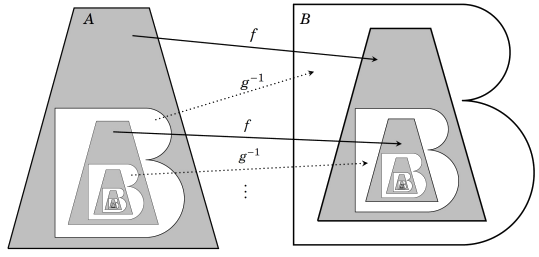
\includegraphics[width=0.7\linewidth]{Iterate}
            %\caption{}
			\label{fig:iterate}
		\end{figure}
	}
}
\end{frame}
\begin{frame}
    \frametitle{Exercise}
    3. Prove the following equinumerosity:
    \begin{itemize}
        \item $\bZ\es\bN$
        \item $\bN \times \bN \es \bN$
        \item $(0,1) \es \bR$
        \item $[0,1] \es (0,1)$
        \item $\calP (\bN) \es \bR$
        \item $\bN^\bN \es \bR$
    \end{itemize}
    \vs{1em}
    \begin{block}{Thinking}
        \begin{itemize}
            \item Could you find a continous bijection?
            \item If not, why?
        \end{itemize}
    \end{block}

\end{frame}
\begin{frame}
    \frametitle{Proof: $\bN^\bN \es \bR$}
    \hh We have $2^{\aleph_0} \leq 3^{\aleph_0} \leq 4^{\aleph_0} \leq \dots \leq \aleph_0^{\aleph_0}$, because of the inclusions $\{0, 1\}^\bN \subset \{0,1,2\}^\bN \subset \dots \subset \bN^\bN$. 
    So if we prove that $\aleph_0^{\aleph_0} \leq 2^{\aleph_0}$, then we see that all of these cardinalities are in fact equal. 
    \\\vs{0.5em}
    \hh To show this, we need to find some injection $f: \bN^{\bN} \to \{0, 1\}^\bN$. There are many ways to do this; my favorite is as follows. Let $a = (a_n)$ be some sequence of natural numbers. 
    Then we define $f\,(a)$ to be the sequence consisting of first $a_0$ ones, followed by a zero, then $a_1$ ones, followed by a zero, then $a_2$ ones, followed by a zero, and so on. 
    This gives a sequence of zeroes and ones, and if $b = (b_n)$ is another sequence of natural numbers, then $f\,(a) = f\,(b)$ if and only if $a_n =b_n$ for all indices $n$ if and only if $a = b$. So $f$ is indeed injective, 
    and therefore $\aleph_0^{\aleph_0} \leq 2^{\aleph_0}$.
    \\\vs{0.5em}
    \hh So indeed $2^{\aleph_0} = 3^{\aleph_0} = \dots = \aleph_0^{\aleph_0}$. 
\end{frame}
\begin{frame}
    \frametitle{Thinking (I don't know don't ask me)}
    A strange thought, why the previous one is wrong?
    \begin{itemize}
        \item Consider $\bN^2,\bN^3,\dots$ is all countable, so $\bN^\bN$ is also countable.
        \item Consider $2^\bN,3^\bN,\dots$ is all equinumerous to $\bR$, so $\bN^\bN$is also equinumerous to $\bR$.
    \end{itemize}
    \vv
    What does these mean?\\
    $$\text{card } \bN = \al ~~~~~\text{card }\bR = \all ~~~~~ \text{card } \bR^\bR = \aleph_2$$

\end{frame}
\section{Finite Sets}
\begin{frame}
    \frametitle{Pigeonhole Principle}
    \yellow{Two versions¿:}
    \vv 
    \begin{enumerate}
        \item[2y/o] Let $r,s \in \mathbb{N} \backslash\!\left\lbrace 0 \right\rbrace $, 
        if a set containing at least ${rs} + 1$ elements is partitioned into $r$ subsets, 
        then some subsets contains at least $s + 1$ elements.
        \item[20y/o] No set of the form $[n] = \left\lbrace 1, \cdots, n\right\rbrace$ 
        is equinumerous to a proper subset of itself, 
        where $n \in \mathbb{N}$.
	\end{enumerate}
\end{frame}
\begin{frame}
    \frametitle{Exercise}
    4. Consider a sequence $\left\lbrace \sqrt{3}, 2\sqrt{3}, 3\sqrt{3}, \cdots \right\rbrace$.
    Prove that there are infinite number of terms have a mantissa of less than 0.01.
    

\end{frame}
\begin{frame}
    \frametitle{Finite Set}
    Important results:
    \begin{itemize}
        \item Let $A$ be any finite set. 
        $f : A \to A$, $f$  injective $\LRarrow$ f
        surjective.
        \item No finite set is equinumerous to a proper subset of itself.
    \end{itemize}
    \vv
    \red{Try to understand them! This may appear in the exam!}
\end{frame}
\begin{frame}
    \frametitle{Longest Increasing Subsequence}
    5. Find the longest increasing/decreasing sequence.
    $$\text{nums }= [10, 9, 2, 5, 3, 7, 101, 18]$$
    \begin{block}{Methodology}
        \begin{table}[]
            \begin{tabular}{||c|ccccccc||}
            \toprule
            num.&0  &1  &2  &3  &4  &5  &6  \\ 
            \midrule
            val.&10  &9  &2  &5  &7  &101  &18  \\ \hline
            len.&1  &1  &1  &2  &3  &4  &4  \\ \hline
            pre.&-  &-  &-  &2  &3  &4  &4  \\ 
            \bottomrule
            \end{tabular}
            \end{table}
    \end{block}
\end{frame}

\section{End}

\begin{frame}
    \frametitle{Reference}

    \begin{itemize}
        \item Figures from 2023-Summer-Ve203 Lecture.
        \item Exercises from 2021-Fall-Ve203 TA Zhao Jiayuan
        \item What-is-the-result-of-a-number-greater-than-2-raised-to-the-power-of-aleph-0
        \url{https://math.stackexchange.com/questions/1646830}
    \end{itemize}

\end{frame}
\begin{frame}
    \frametitle{}

    \begin{center}
        \Huge{$\mathcal{THANKS}$!}
    \end{center}

\end{frame}
\end{document}